\documentclass{jlreq}

\usepackage{fontspec}
\usepackage{unicode-math}
\setmainfont{Latin Modern Roman}
\setmathfont{Latin Modern Math}
\usepackage{pgfplots}
\pgfplotsset{compat=1.18}
\usepgfplotslibrary{statistics}

\begin{document}

これはテストです。English and math: \( \frac{\sin r}{r} \)

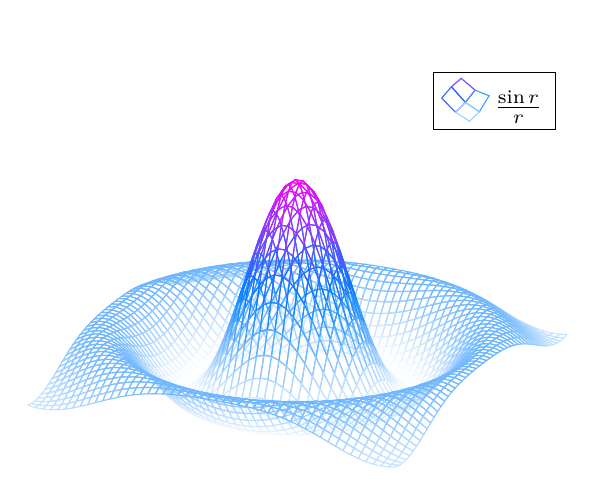
\begin{tikzpicture}
\begin{axis}[
    title=グラフタイトル,
    colormap/cool,
    hide axis,
]
\addplot3[
    mesh,
    samples=50,
    domain=-8:8,
]
{sin(deg(sqrt(x^2+y^2)))/sqrt(x^2+y^2)};
\addlegendentry{$\frac{\sin r}{r}$}
\end{axis}
\end{tikzpicture}

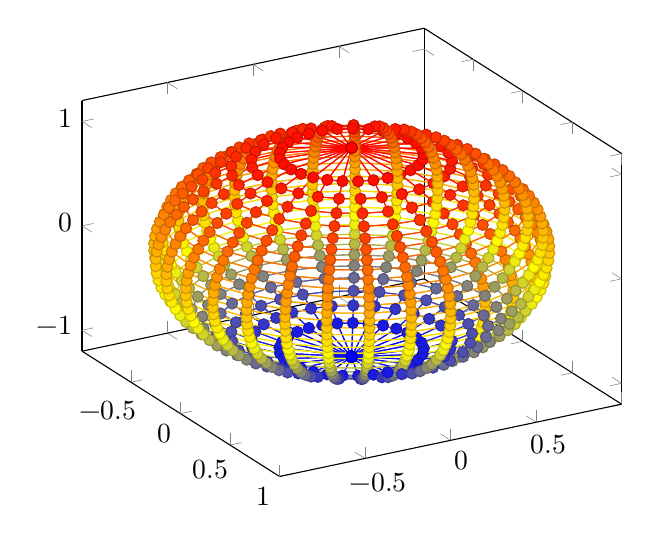
\begin{tikzpicture}
\begin{axis}[view={60}{30}]
\addplot3 [
only marks,
mesh,z buffer=sort,
scatter,scatter src=z,
samples=30,domain=-1:1,y domain=0:2*pi,
] (
{sqrt(1-x^2) * cos(deg(y))},
{sqrt( 1-x^2 ) * sin(deg(y))},
x
);
\end{axis}
\end{tikzpicture}

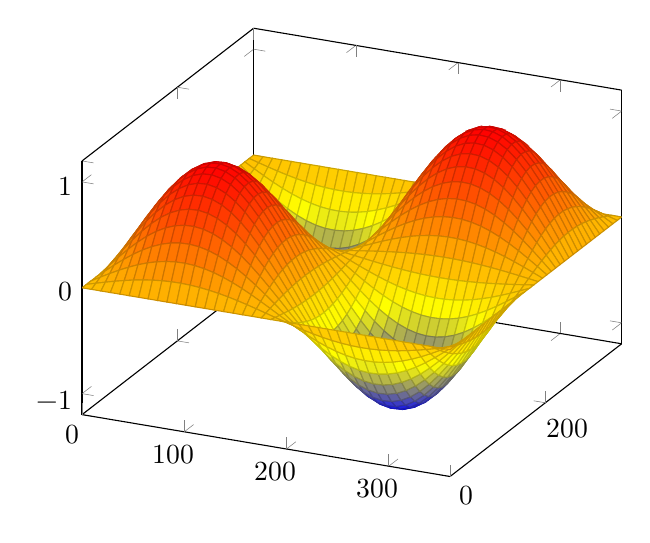
\begin{tikzpicture}
\begin{axis}
\addplot3 [
surf,
domain=0:360,
samples=40,
] {sin(x)*sin(y)};
\end{axis}
\end{tikzpicture}




\end{document}
